\RequirePackage[l2tabu, orthodox]{nag}
% \documentclass[handout]{beamer}
\documentclass{beamer}
\usetheme{metropolis}
\usepackage{appendixnumberbeamer}

\usepackage{booktabs}
\usepackage[scale=2]{ccicons}

% makes table of contents and such hyperlinks
\usepackage{hyperref}

\usepackage[style=authoryear, hyperref = true]{biblatex}
\addbibresource{library.bib}

\setbeamercolor{background canvas}{bg=white}
\newcommand\blfootnote[1]{%
  \begingroup
  \renewcommand\thefootnote{}\footnote{#1}%
  \addtocounter{footnote}{-1}%
  \endgroup
}

\setlength{\leftmargini}{12pt}
\usetikzlibrary{arrows, shapes, positioning}

\usepackage{xspace}
\usepackage{commath}
\usepackage{graphics}
\usepackage{algorithm2e}
\DeclareMathOperator*{\argmax}{argmax}

\title{Using reinforcement learning to personalize dosing strategies in a simulated cancer trial with high dimensional data}
\subtitle{\sl or: how I learned to stop worrying and love creating billion-observation data frames}
\date{\today}
\author{Kyle Humphrey}
\institute{University of Arizona}
% \titlegraphic{\hfill\includegraphics[height=1.5cm]{logo.pdf}}

\begin{document}

\maketitle

\begin{frame}[c]{Table of contents}
  \setbeamertemplate{section in toc}[sections numbered]
  \tableofcontents
\end{frame}

\section{Introduction}

\subsection{Personalized medicine} % (fold)
\label{sub:personalized_medicine}

\begin{frame}[c]{Personalized medicine}

Patients often have different responses to treatment
\begin{itemize}[<+(1)->]
  \item Adverse drug reactions alone are significant burden 
  \begin{itemize}
    \item 6.5\% of hospital admissions at two hospitals in England  (\cite{Pirmohamed2004})
    \item Projected to cost NHS \$850 million annually 
  \end{itemize}
  \item Other factors increase patient response
  \begin{itemize}
    \item Whether breast cancer cells over-express human epidermal growth factor receptor 2 (are HER2-positive)\footnotemark 
  \end{itemize}
\end{itemize}

\only<6->{\footnotetext{Usually, ``personalized medicine'' refers to this type of biomarker-based personalization}}

\end{frame}

\begin{frame}[c]{How to personalized medicine?}

Identify subgroups who respond to treatment differently
\begin{itemize}[<+(1)->]
  \item Treatment by covariate interactions
  \begin{itemize}
    \item Problem: Lots of potential subgroups/interactions
    \begin{itemize}
      \item Need lots of data (and)
      \item Method for multiple comparisons
    \end{itemize}
  \end{itemize}
  \item Lots of novel methods
  \begin{itemize}
    \item Problems (in our setting): 
    \begin{itemize}
      \item Treatments always categorical
      \item \textbf{Only single stage considered}
    \end{itemize}
  \end{itemize}
\end{itemize}

\end{frame}

% subsection personalized_medicine (end)

\begin{frame}[c]{Broad overview}

Goal: find sequence of doses of a single treatment that maximize survival time in a simulated cancer clinical trial\footnote{setup inspired by \textcite{crt}} with and without high dimensional covariates and patient subgroups
\begin{itemize}[<+(1)->]
    \item Use Q-learning, an algorithm from reinforcement learning
    \item To fit Q-functions: 
    \begin{itemize}[<+->]
      \item Regression trees (CART--\cite{CART})
      \item Multivariate adaptive regression splines (MARS--\cite{mars})
      \item Random forest (RF--\cite{rf})
    \end{itemize} 
\end{itemize}

\end{frame}
%--- Next Frame ---%

\section{Reinforcement learning} % (fold)
\label{sec:reinforcement_learning}

\begin{frame}[c]{Reinforcement learning: sequential decision making}
  \begin{figure}
    \centering
    \includegraphics[width = 0.68\textwidth]{figure/rl-venn-silver}
    \blfootnote{\scriptsize Image by \href{http://www0.cs.ucl.ac.uk/staff/D.Silver/web/Teaching.html}{David Silver}}
  \end{figure}
\end{frame}
%--- Next Frame ---%

\begin{frame}[c]{Reinforcement learning: basic elements}

\begin{itemize}[<+->]
  \item \emph{Agent} who has goal(s) regarding
  \item \emph{Environment} (everything outside agent's direct control)
  \begin{itemize}
    \item Features of environment represented via \emph{states}
  \end{itemize}
  \item Agent follows \emph{policy}: 
  \begin{itemize}
    \item \emph{Action} to take in a given state to achieve goal(s)
    \item (Reward hypothesis): maximizing scalar, \emph{reward}, achieves goal(s) 
  \end{itemize}
  \item Reinforcement learning: find \emph{optimal policy}--policy achieves largest reward over long run 
\end{itemize}

\end{frame}
%--- Next Frame ---%

\begin{frame}[c]{Reinforcement learning: basic process}
\begin{columns}%[<options>]
  \begin{column}{0.54\textwidth}
        \centering
    \includegraphics[width=\textwidth]{figure/rl-process} \\*
        \vspace{-6pt}
        \hrulefill \\*
        \vspace{-6pt}
        {\scriptsize Image by \href{http://www0.cs.ucl.ac.uk/staff/D.Silver/web/Teaching.html}{David Silver}}
  \end{column}
  \begin{column}{0.5\textwidth}
    Agent:
    \begin{enumerate}[<+->]
      \item Presented with states $O_{t}$
      \item Tries action $A_{t}$
      \item Gets reward $R_{t}$
      \item Estimates relationship between $A_{t}$, $O_{t}$, and $R_{t}$
      \item Chooses $A_{t+1}$ that leads to largest rewards
    \end{enumerate}
  \end{column}
\end{columns}
\end{frame}
%--- Next Frame ---%

% \begin{frame}[c]{Reinforcement learning: example}
%
% \begin{itemize}
%     \item States: the positions of the pieces on the board
%     \item Actions: any of the legal moves with any given piece
%     \item Rewards: e.g. \\
%     if win $reward \gets 1$ \\
%     if lose $reward \gets 0$
%     \item Policy: ``strategy''
% \end{itemize}
%
% AlphaGo uses reinforcement learning and neural networks
%
% \end{frame}
% %--- Next Frame ---%


\begin{frame}[t]{Reinforcement learning: basic process}

\end{frame}
%--- Next Frame ---%

\begin{frame}[c]{Reinforcement learning: relationship to other areas of machine learning}
\begin{itemize}[<+->]
  \item Supervised learning
  \begin{itemize}
    \item Agent given correct example actions to take
    \item Goal: agent extrapolates correct behavior to new situations
  \end{itemize}
  \item Unsupervised learning
  \begin{itemize}
    \item Agent given example actions where correct action unknown
    \item Goal: agent finds hidden structure
  \end{itemize} 
  \item Reinforcement learning
\begin{itemize}
  \item No correct example actions required
  \item Goal: maximize rewards, not find hidden structure
  \item Feedback delayed 
  \item Problems closed loop: actions taken now affect available actions and rewards later
\end{itemize} 
\end{itemize}
\end{frame}
%--- Next Frame ---%


\begin{frame}[c]{Reinforcement learning: connection to personalized medicine}
  
  \begin{itemize}[<+->]
      \item States: patient histories and characteristics
      \item Actions: possible treatment options
      \item Rewards: goal dependent (e.g. kg weight lost in weight loss study)
      \item Policy: \emph{dynamic treatment regime} 
  \end{itemize}

\end{frame}
%--- Next Frame ---%

\subsection{Q-learning} % (fold)
\label{sub:q_learning}

\begin{frame}{Q-learning: setup (\cite{dtr-review})}
  Patients recruited into a trial,
  \begin{enumerate}[<+(1)->]
    \item Covariates measured $\rightarrow O_{0}$ \\*
    Patient history stage 0: $H_{0} \doteq O_{0}$
    \item Treatment $A_{0}$ randomly assigned
    \item Covariates measured $\rightarrow O_{1}$ \\*
    Reward $R_{1}$ received \\*
    Patient history stage 1: $H_{1} \doteq (O_{0}, A_{0}, O_{1})$
    \item Treatment $A_{1}$ randomly assigned (could depend on $H_{1}$)
    \item Covariates measured $\rightarrow O_{2}$ \\*
    Reward $R_{2}$ received \\*
    $H_{2} \doteq (H_{1}, A_{1}, O_{2})$
  \end{enumerate}
    \pause
    process repeated over $K$ stages
\end{frame}
%--- Next Frame ---%

\begin{frame}{Example setup: my simulation}
\resizebox{\textwidth}{!}{
     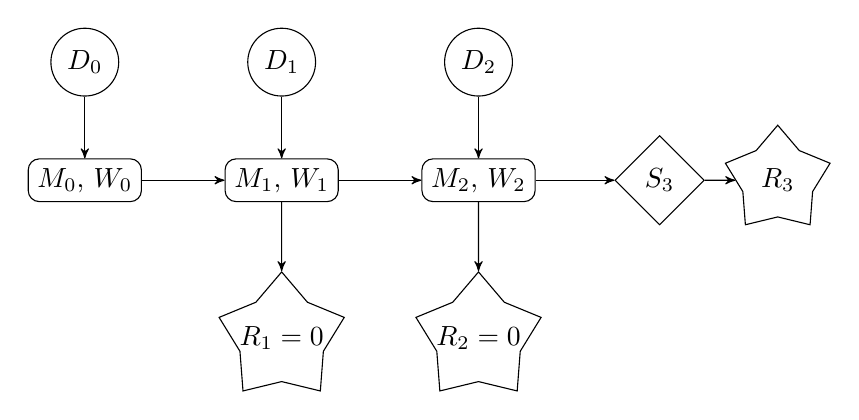
\begin{tikzpicture}[->, >=stealth', auto, node distance=1.5cm, minimum size=1pt,
    pt node/.style={rounded corners, draw},
    pt node img/.style={rounded corners, dashed, draw},
    dose node/.style={circle, draw},
    surv node/.style={diamond, draw},
    r node/.style={star, draw}]

    \node[pt node]    (M0) {$M_{0}$, $W_{0}$};
    \node[dose node]  (D0) [above of = M0] {$D_{0}$};
    \path (D0) edge (M0);
    
    \pause
    
    \node[pt node]    (M1) [right of = M0, xshift = 1cm] {$M_{1}$, $W_{1}$};
    
    \node[r node]     (R1) [below of = M1, inner sep = -4pt, yshift = -0.5cm] {$R_{1} = 0$};
    \path (M0) edge (M1) (M1) edge (R1);

    \pause
    
    \node[dose node]  (D1) [above of = M1] {$D_{1}$};
    \path (D1) edge (M1);
    
    \pause
    
    \node[pt node] (M2) [right of = M1, xshift = 1cm] {$M_{2}$, $W_{2}$};
    \path (M1) edge (M2);
    \node[r node]     (R2) [below of = M2, inner sep = -4pt, yshift = -0.5cm] {$R_{2} = 0$};
    \path (M2) edge (R2);
    
    \pause
    
    \node[dose node]  (D2) [above of = M2] {$D_{2}$};
    \path (D2) edge (M2);
    
    \pause
    
    \node[surv node]  (S3) [right of = M2, xshift = 0.8cm] {$S_{3}$};
    \node[r node]     (R3) [right of = S3] {$R_{3}$};
    \path (M2) edge (S3) (S3) edge (R3);
  \end{tikzpicture}
  }
\end{frame}

\begin{frame}[c]{Q-learning}
  Q-function at stage $k$
    \begin{equation*}
       Q_{k}(A_{k}, H_{k})  = \operatorname{E}[R_{k} \mid A_{k}, H_{k}], \quad k = 0, \ldots, K
    \end{equation*}
        %
        \pause
        %
\begin{algorithm}[H]
  $\hat{Q}_{K + 1} \gets 0$

  \medskip

 \For{$k$ in $K, \ldots, 0$}{
  Make outcome rewards if optimal policy followed after $k$:

$\hat{R}_{k} \gets R_{k} + \max_{A_{k+1}} \hat{Q}_{k+1}(A_{k+1}, H_{k+1})$

\medskip

Estimate Q-function, $Q_{k}(A_{k}, H_{k})$, for stage $k$ using $\hat{R}_{k}$

\medskip

Estimate the optimal treatment for each patient at stage $k$:

$\hat{A}^{opt}_{k} \gets \argmax_{A_{k}} \hat{Q}_{k}(A_{k}, H_{k})$
}
\end{algorithm}
\end{frame}
%--- Next Frame ---%


\begin{frame}{Q-learning example: my simulation}
\resizebox{1.1\textwidth}{!}{
     \begin{tikzpicture}[->, >=stealth', auto, node distance=1.5cm, minimum size=1pt,
    pt node/.style={rounded corners, draw},
    pt node img/.style={rounded corners, dashed, draw},
    dose node/.style={circle, draw},
    surv node/.style={diamond, draw},
    r node/.style={star, draw}]

    \node[pt node]    (M0) {$M_{0}$, $W_{0}$};
    \node[dose node]  (D0) [above of = M0] {$D_{0}$};
    \path (D0) edge (M0);
    \node[pt node]    (M1) [right of = M0, xshift = 1cm] {$M_{1}$, $W_{1}$};
    \node[r node]     (R1) [below of = M1, inner sep = -4pt, yshift = -0.5cm] {$R_{1} = 0$};
    \path (M0) edge (M1) (M1) edge (R1);
    \node[dose node]  (D1) [above of = M1] {$D_{1}$};
    \path (D1) edge (M1);
    \node[pt node] (M2) [right of = M1, xshift = 1cm] {$M_{2}$, $W_{2}$};
    \path (M1) edge (M2);
    \node[r node]     (R2) [below of = M2, inner sep = -4pt, yshift = -0.5cm] {$R_{2} = 0$};
    \path (M2) edge (R2);
    \node[dose node]  (D2) [above of = M2] {$D_{2}$};
    \path (D2) edge (M2);
    \node[surv node]  (S3) [right of = M2, xshift = 0.8cm] {$S_{3}$};
    \node[r node]     (R3) [right of = S3] {$R_{3}$};
    \path (M2) edge (S3) (S3) edge (R3);
    
    \pause
    \draw [->, dashed] (R3) edge (Q3);
    \node (Q3) [below right of = R3] {$\hat{R}_{3} = R_{3}$};
    % (M2) edge [bend right = 30] (Q3)
    
    \pause
    
    \draw [->, dashed] (Q3) edge [bend right = 30] node {$\hat{Q}_{3} = \operatorname{E}[\hat{R}_{3}|D_{2}, M_{2},W_{2}]$} (Q2);

    \pause
    
    \node (Q2) [below right of = R2, xshift = 1cm, yshift = -0.5cm] {$\hat{R}_{2} = R_{2} +  \max_{D_{2}} \hat{Q}_{3}$};
    \draw [->, dashed] (R2) edge (Q2);
    
    \pause
    
    \draw [->, dashed] (Q2) edge [bend left = 30] node {$\hat{Q}_{2} = \operatorname{E}[\hat{R}_{2}|D_{1}, M_{1},W_{1}]$} (Q1);

    \pause
   
    \node (Q1) [below right of = R1, yshift = -1cm, xshift = -1cm] {$\hat{R}_{1} = R_{1} +  \max_{D_{2}} \hat{Q}_{1}$};
    \draw [->, dashed] (R1) edge (Q1);
    
    \pause
    
    \node (Q0) [below of = M0, yshift = -3.5cm, xshift =1cm] {$\hat{Q}_{1} = \operatorname{E}[\hat{R}_{1}|D_{0}, M_{0},W_{0}]$};
    
    \draw [->, dashed] (Q1) edge (Q0);

  \end{tikzpicture}
  }
\end{frame}

% subsection q_learning (end)

% section reinforcement_learning (end)

\section{Methods to fit Q-functions} % (fold)
\label{sec:methods_to_fit_q_functions}

\begin{frame}[c]{Why trees (and MARS)?}
  \begin{itemize}[<+->]
    \item ``Automatically'' conduct variable selection and interaction modelling
    \item Not restricted to linear relationships between $X$ and $Y$
    \item Produce interpretable models 
    \item Are similar to each other and easier for me to explain 
  \end{itemize}
\end{frame}
%--- Next Frame ---%

\subsection{Regression trees (CART)} % (fold)
\label{sub:cart}

\begin{frame}{Regression trees (CART): example}
  For 50 patients with initial tumor mass $M_{0} \overset{iid}{\sim} \text{Unif}(1, 2)$,
  \begin{itemize}[<+(1)->]
    \item Predict change in tumor mass: $Y_{i} \doteq M_{i1} - M_{i0}$ \\* given dose of treatment $D_{i}$ assigned
    \item True relationship:
    \begin{align*}
      Y_{i} &= 0.75 - 1.2 D_{i} + \epsilon_{i}, \quad i = 1, \ldots, 50 \\
      & \epsilon_{i} \sim N(0, 0.05)
    \end{align*}
  \end{itemize}
\end{frame}
%--- Next Frame ---%

\begin{frame}[c]{Regression trees (CART): example tree}
  \begin{figure}[!htbp]
  \begin{center}
    \includegraphics[width=\textwidth]{figure/ex-cart-tree-1}
  \end{center}
  \end{figure}
\end{frame}
%--- Next Frame ---%

\begin{frame}{Regression trees (CART): tree growing}
  Goal: make nodes as homogeneous in outcome as possible
  
  \pause
  Need to decide:
  \begin{enumerate}[<+->]
    \item What covariate to use to define split and what value of the covariate to split on
    \item When to stop splitting
    \item How to assign outcomes to terminal nodes
  \end{enumerate}
\end{frame}
%--- Next Frame ---%

\begin{frame}{Regression trees (CART): tree growing}
  Start with root node
  
  \begin{enumerate}[<+(1)->]
  \item Try splitting each unique value $x_{ij}$ of each covariate $X_{j}$
  \item Calculate the resulting $SSE$
  \begin{equation*}
    SSE = \sum_{i \in \text{node}_{L}} (y_{i} - \bar{y}_{L})^2 + \sum_{i \in \text{node}_{R}} (y_{i} - \bar{y}_{R})^2
  \end{equation*}
  $\bar{y}_{L} = $ average outcome in left node, $\text{node}_{L}$, and \\*   $\bar{y}_{R} = $ average outcome in right node, $\text{node}_{R}$.
  \item Pick split that minimizes $SSE$
    \end{enumerate}
  \pause
  Repeat for resulting nodes 
    
  \begin{itemize}[<+(1)->]
  \item Stop splitting once e.g. resulting nodes too small
  \item Average outcome in each terminal node predicted outcome 
  \end{itemize}
\end{frame}
%--- Next Frame ---%

\begin{frame}[c]{Regression trees (CART): tree pruning}
  \begin{itemize}[<+->]
    \item Result is bushy/deep tree $T_{0}$ that overfits
    \item Cost-complexity pruning: find subtrees $T \subset T_{0}$ that minimize
    \begin{equation*}
        C_{\alpha}(T) = \sum_{m = 1}^{\abs{T}} \sum_{x_{i} \in \text{node}_{m}} (y_{i} - \bar{y}_{m})^2 + \alpha \abs{T}
    \end{equation*}
    \item Unique subtree $T_{\alpha}$ that minimizes $C_{\alpha}(T)$ for each $\alpha \geq 0$.
  \end{itemize}
\end{frame}
%--- Next Frame ---%

\begin{frame}[c]{Regression trees (CART): tree pruning}
  Find $T_{\alpha}$ using weakest link pruning
      \begin{enumerate}[<+(1)->]
        \item Try collapsing each internal node in turn
        \item Actually collapse weakest link \\*
        (collapsing node $\rightarrow$ smallest increase in $SSE$) \\*
         save tree
        \item Repeat to root node 
      \end{enumerate}
      
      \begin{itemize}[<+(1)->]
        \item In saved trees: sequence of $T_{\alpha}$s (best trees of given size)
        \item Choose final tree from $T_{\alpha}$s using resampling technique
      \end{itemize}
      

\end{frame}
%--- Next Frame ---%

\begin{frame}[c]{Regression trees (CART): example tree}
  \begin{figure}[!htbp]
  \begin{center}
    \includegraphics[width=\textwidth]{figure/ex-cart-tree-1}
  \end{center}
  \end{figure}
\end{frame}
%--- Next Frame ---%

\begin{frame}{Regression trees (CART) example function}
  \begin{figure}[!htbp]
  \begin{center}
    \includegraphics[width=0.9\textwidth]{figure/ex-plot-cart-1}
  \end{center}
  \end{figure}
\end{frame}
%--- Next Frame ---%

% \begin{frame}{Regression trees (CART)}
%   Why we like trees:
%   \begin{enumerate}
%     \item Easy to interpret
%     \item Feature selection and modelling of interactions part of process
%     \item Easy to handle many types of covariates without pre-processing
%   \end{enumerate}
%
%   Why we don't like trees:
%   \begin{enumerate}
%     \item Generally have lower performance than other methods, particularly in regression setting
%   \end{enumerate}
% \end{frame}
% %--- Next Frame ---%

% subsection cart (end)

\subsection{MARS} % (fold)
\label{ssub:mars}

\begin{frame}{Multivariate Adaptive Regression Splines}
  \begin{itemize}[<+->]
    \item Generalization of stepwise linear regression methods that incorporates modelling interactions
    \item Model covariates as piecewise linear basis functions:
  %
  \begin{equation*} \label{eq:bases}
    (x - t)_{+} \text{ and } (t - x)_{+}
  \end{equation*} where
  %
  \begin{equation*}
    (Z)_{+} = \max(Z, 0) = \begin{cases}
    Z, & \text{if } Z > 0 \\
    0, & \text{otherwise}
    \end{cases}
  \end{equation*}
  \end{itemize}
\end{frame}
%--- Next Frame ---%

\begin{frame}{Multivariate Adaptive Regression Splintes}
  \begin{itemize}
    \item Generalization of stepwise linear regression methods that incorporates modelling interactions
    \item Model covariates as piecewise linear basis functions:
  %
  \begin{equation*} \label{eq:bases}
    \underbrace{(x - t)_{+}}_\text{hinge function} \text{ and } \underbrace{(t - x)_{+}}_\text{hinge function}
  \end{equation*} where
  %
  \begin{equation*}
    (Z)_{+} = \max(Z, 0) = \begin{cases}
    Z, & \text{if } Z > 0 \\
    0, & \text{otherwise}
    \end{cases}
  \end{equation*}
  \end{itemize}
\end{frame}
%--- Next Frame ---%

\begin{frame}{Multivariate Adaptive Regression Splintes}
  \begin{itemize}
    \item Generalization of stepwise linear regression methods that incorporates modelling interactions
    \item Model covariates as piecewise linear basis functions:
  %
  \begin{equation*} \label{eq:bases}
    \underbrace{(x - t)_{+}}_\text{linear spline} \text{ and } \underbrace{(t - x)_{+}}_\text{linear spline}
  \end{equation*} where
  %
  \begin{equation*}
    (Z)_{+} = \max(Z, 0) = \begin{cases}
    Z, & \text{if } Z > 0 \\
    0, & \text{otherwise}
    \end{cases}
  \end{equation*}
  \end{itemize}
\end{frame}
%--- Next Frame ---%


\begin{frame}{Multivariate Adaptive Regression Splintes}
  \begin{itemize}
    \item Generalization of stepwise linear regression methods that incorporates modelling interactions
    \item Model covariates as piecewise linear basis functions:
  %
  \begin{equation*} \label{eq:bases}
    (x - \overbrace{t}^\text{knot})_{+} \text{ and } (\overbrace{t}^\text{knot} - x)_{+}
  \end{equation*} where
  %
  \begin{equation*}
    (Z)_{+} = \max(Z, 0) = \begin{cases}
    Z, & \text{if } Z > 0 \\
    0, & \text{otherwise}
    \end{cases}
  \end{equation*}
  \end{itemize}
\end{frame}
%--- Next Frame ---%

\begin{frame}{MARS: Model building (forward pass)}
  
  \begin{itemize}[<+->]
    \item As in forward selection, start with constant
    \begin{equation*}
      f(X) = \beta_{0}
    \end{equation*}
    \item Consider adding pairs of piecewise linear functions:
  \begin{equation*}
  \beta_{1} (X_{j} - x_{ij})_{+} + \beta_{2}(x_{ij} - X_{j})_{+}, \ i = 1, 2, \ldots, n; \ j = 1, 2, \ldots, p.
  \end{equation*}
   For each covariate $X_{j}$ split at an observed value, $x_{ij}$
  \begin{enumerate}
    \item Try adding each possible pair to the model
    \item Calculate the $SSE$
    \item Add pair that minimizes $SSE$
  \end{enumerate}
  \end{itemize}

\end{frame}
%--- Next Frame ---%

\begin{frame}{MARS: Model building (forward pass)}
  \begin{itemize}[<+->]
    \item Then consider adding pairs with general form:
  \begin{equation*} \label{eq:gen-pairs-add}
    \beta_{M + 1} h_{\ell}(X) \cdot (X_{j} - x_{ij})_{+} + \beta_{M + 2} h_{\ell}(X) \cdot (x_{ij} - X_{j})_{+}
  \end{equation*}
  $h_{\ell}(X) = $ hinge function (or product of hinge functions) already in model\footnote{Also holds for the first step where $h_{\ell}(X) = h_{0}(X) = 1$}
  \item Add pair that minimizes $SSE$
  \item Repeat until 
  \begin{itemize}
    \item Change in $SSE$ too small and/or
    \item Too many terms in model
  \end{itemize}
  \end{itemize}
\end{frame}
%--- Next Frame ---%

\begin{frame}{MARS: Backward pass}
  \begin{itemize}[<+->]
    \item Resulting model usually overfits
    \item As in backward selection, remove terms from model one by one:
    \begin{enumerate}
      \item Record $SSE$ increase by removing each term in turn
      \item Remove term that increases $SSE$ the least
      \item Repeat until no terms left
    \end{enumerate}
    \item Result of each stage: $\hat{f}_{\lambda}(X)$, best model with $\lambda$ terms
  \end{itemize}

\end{frame}
%--- Next Frame ---%

\begin{frame}{MARS: Backward pass}
Pick final model ($\lambda$) using generalized cross validation (GCV) 
    
    \pause
    
    \begin{equation*}
    GCV(\lambda) =
      \frac{
        \sum_{i = 1}^{N}(y_{i} - \hat{f}_{\lambda}(x_{i}))^2
      }{
        (1 - M(\lambda)/N)^2
      }
  \end{equation*}
  %
  \begin{align*}
    M(\lambda) &= \lambda + 3(\text{\# knots}) \\
     &=\lambda + 2(\text{\# knots}) \quad \text{when restricted to additive}
  \end{align*}
\end{frame}
%--- Next Frame ---%

% \begin{frame}{MARS: Relationship to CART}
%   \begin{itemize}[<+->]
%     \item MARS: modification of CART to improve regression performance
%     \item MARS forward pass $\equiv$ CART tree growing if:
%     \begin{enumerate}[<+->]
%       \item Change hinge functions to step functions:
%       \begin{equation*}
%         I(x - t > 0) \text{ and } I(t - x > 0)
%       \end{equation*}
%       \item Replace term in model involved in new interaction by new interaction \\*
%       (original term unavailable for future interactions)
%     \end{enumerate}
%   \end{itemize}
% \end{frame}
% %--- Next Frame ---%


\begin{frame}[t]{MARS: example}

\begin{figure}[!htbp]
\begin{center}
  \includegraphics[width=0.9\textwidth]{figure/ex-plot-mars-1}
\end{center}
\end{figure}
%
\begin{equation*}
  \label{eq:mars-eqn}
  \hat{f}(D) \approx -0.24 + 1.24 (0.81 - D)_{+} -1.64 (D - 0.87)_{+}
\end{equation*}

\end{frame}
%--- Next Frame ---%

% subsubsection mars (end)

\subsection{Bagging and Random Forest} % (fold)
\label{sub:bagging_and_random}

\begin{frame}{Bagging}
  
  \begin{itemize}[<+->]
    \item Single trees: high variance \\* 
    (small changes in data $\rightarrow$ very different trees)
    \item When trees deep/bushy $\rightarrow$ relatively low bias 
  \end{itemize}
\end{frame}
%--- Next Frame ---%

\begin{frame}{Bagging}
  
  \begin{itemize}[<+->]
    \item Consider iid random variables, $X_{1}, X_{2}, \ldots, X_{n}$, each with variance $\sigma^2$ and sample mean $\bar{X}$:
  \begin{equation*}
    \operatorname{Var}[\bar{X}] = \frac{\sigma^2}{n}
  \end{equation*}
  \item Improve tree performance by building trees on many different samples then averaging results!
  \item Problem: only have one sample
  \end{itemize}
\end{frame}
%--- Next Frame ---%

\begin{frame}[c]{Bagging}
  Do bootstrap aggregating (\emph{bagging}):
  \begin{enumerate}[<+->]
    \item Take $B$ bootstrap resamples of sample
    \item Fit model to each resample (grow a tree, don't prune)
    \item Average the resulting predictions
    \item Make profit 
  \end{enumerate}
\end{frame}
%--- Next Frame ---%

\begin{frame}{Random forest}
  Problem: trees are correlated: can't reduce variance $B$ fold
  \begin{itemize}[<+->]
    \item \textcite{rf}: decrease correlation by 
    \begin{itemize}
      \item only consider random $m_{try} \subset p$ predictors for splitting at each split
    \end{itemize}
    \item Choose $m_{try}$ using resampling techniques
    \item Performance much better than single tree, \\* but also much less interpretable
  \end{itemize}
\end{frame}
%--- Next Frame ---%

\begin{frame}{Random forest (bagging) example}
  
  \begin{figure}[!htb]
  \begin{center}
    \includegraphics[width=0.9\textwidth]{figure/ex-plot-rf-1}
  \end{center}
  \end{figure}
  
\end{frame}
%--- Next Frame ---%

% subsection bagging_and_random (end)

% section methods_to_fit_q_functions (end)

\section{Simulation} % (fold)
\label{sec:simulation}

\begin{frame}[c]{Setup}
  \begin{itemize}[<+->]
    \item 1000 patients
    
  \item Initial toxicity, $W_{0} \equiv$ -wellness $\equiv$ -quality of life
  \begin{equation*}
    W_{0} \overset{iid}{\sim} \text{Unif}(0, 2)
  \end{equation*}
  
  \item Initial tumor mass, $M_{0}$
  \begin{align*}
    M_{0} &\overset{iid}{\sim} \text{Unif}(0, 2)
  \end{align*}
  
  \item Treatment: three random doses, one each month
  \begin{align*}
    D_{t} &\overset{iid}{\sim} \text{Unif}(0, 1), \quad t = 0, 1, 2
  \end{align*}
  ($D = 0$: none; $D = 1$: maximum tolerable)
  \end{itemize}
\end{frame}
%--- Next Frame ---%

\begin{frame}[c]{Patient model: transition functions}
  \begin{itemize}[<+->]
    \item Toxicity:
  \begin{equation*}
  W^{*}_{t} = 0.1 M_{t-1} + 1.2 (D_{t-1} - 0.5) + W_{t - 1}
  \end{equation*}
  \begin{equation*}
  W_{t} = \begin{cases}
    W^{*}_{t} &\text{if } W^{*}_{t} > 0 \\
    0 &\text{if } W^{*}_{t} \leq 0
  \end{cases}
  \end{equation*}
  
  \item Tumor mass:
  \begin{equation*}
  M^{*}_{t} = [0.15 W_{t-1} - 1.2 (D_{t-1} - 0.5) + M_{t - 1}] I(M_{t-1} > 0)
  \end{equation*}
  \begin{equation*}
  M_{t} = \begin{cases}
    M^{*}_{t} &\text{if } M^{*}_{t} > 0 \\
    0 &\text{if } M^{*}_{t} \leq 0
  \end{cases}
  \end{equation*}
  \end{itemize}
\end{frame}
%--- Next Frame ---%

\begin{frame}[c]{Patient model: survival}
  \begin{align*}
    \onslide<1->{S^{*}_{it} &\sim \operatorname{exponential}(\beta_{it}(M_{it + 1}, W_{it + 1})) \\[1em]}
    \onslide<2->{\beta_{it}(M_{it+1}, W_{it+1}) &= \exp(5.5 - W_{it+1} - 1.2 M_{it+1} - 0.75 W_{it+1} M_{it+1}) \\[1em]}
   \onslide<3->{S_{it} &= \begin{cases}
      S^{*}_{it} + \sum_{j = 0}^{t} j & \text{if } S_{it} \leq 1 \text{ or } t = 2 \\
      \text{undefined} & \text{otherwise}
    \end{cases} \\[1em]}
   \onslide<4>{R_{it + 1} &=\begin{cases}
          \log(S_{it}) & \text{if } S_{it} \leq 1 \text{ or } t = 2 \\
          0 & \text{otherwise\footnotemark}
        \end{cases}}
  \end{align*}  
  \only<4>{\footnotetext{log survival: continuous reward/outcome, not censored time-to-event}}
\end{frame}
%--- Next Frame ---%

\begin{frame}[c]{Graphs}
  \href{https://www.desmos.com/calculator/bhofs34c6k}{graphs}
\end{frame}
%--- Next Frame ---%

\begin{frame}[c]{Why these functions?}
  \centering
  \includegraphics[width=0.45\textwidth]{figure/cells}
  \bigskip
  \blfootnote{\url{https://xkcd.com/1217/}}
\end{frame}
%--- Next Frame ---%

\begin{frame}[c]{Example patient profile}
  \includegraphics[width=\textwidth]{figure/ind-plot-1} 
\end{frame}
%--- Next Frame ---%

\begin{frame}[c]{Interaction (I) scenario}
  Two additional baseline covariates for each patient:
  \begin{equation*}
    X_{1}, X_{2} \overset{iid}{\sim} \text{Unif}(0, 1)
  \end{equation*}
  
  \begin{itemize}[<+->]
    \item[] $X_{1} < 0.5 \ \& \ X_{2} < 0.5$: same as before
    \item[] $X_{1} > 0.5 \ \& \ X_{2} < 0.5$: 50\% more sensitive to drug effects:
  \begin{equation*}
  W^{*}_{t} = W'_{t} = 0.1 M_{t-1} + 1.2 (\mathbf{1.5} D_{t-1} - 0.5) + W_{t - 1}
  \end{equation*}
  \item[] $X_{1} < 0.5 \ \& \ X_{2} > 0.5$: drug 50\% more effective:
  \begin{equation*}
  M^{*}_{t} =  M'_{t} = [0.15 W_{t-1} - 1.2 (\mathbf{1.5} D_{t-1} - 0.5) + M_{t - 1}] I(M_{t-1} > 0)
  \end{equation*}
  \item[]   $X_{1} > 0.5 \ \& \ X_{2} > 0.5$: 50\% more effective and 50\% more sensitive:
  \begin{align*}
  W^{*}_{t} = W'_{t} &= 0.1 M_{t-1} + 1.2 (\mathbf{1.5} D_{t-1} - 0.5) + W_{t - 1} \\
  M^{*}_{t} = M'_{t} &= [0.15 W_{t-1} - 1.2 (\mathbf{1.5} D_{t-1} - 0.5) + M_{t - 1}] I(M_{t-1} > 0)
  \end{align*}
  \end{itemize}
\end{frame}
%--- Next Frame ---%

\begin{frame}[c]{Noise scenarios}
  \begin{itemize}
    \item Noise (N) scenario: 100 more baseline covariates with no effect:
  \begin{align*}
    Z_{1}, \ldots, Z_{5} &\overset{iid}{\sim} N(1, 1) \\
    Z_{6}, \ldots, Z_{10} &\overset{iid}{\sim} N(-1, 1) \\
    V_{1}, \ldots, V_{90} &\overset{iid}{\sim} N(0, 1)
  \end{align*}
  \item Predictive noise (PN) scenario: same as N but
  %
  \begin{align*}
    \beta'_{it}&(M_{it+1}, W_{it+1}) = \\
    &\exp\del{5.5 + W_{it+1} + 1.2 M_{it+1} + 0.75 W_{it+1} M_{it+1} + 0.05 \sum_{j = 1}^{10} Z_{ij}}
  \end{align*}
  \end{itemize}
\end{frame}
%--- Next Frame ---%

\begin{frame}[c]{Interaction + noise scenarios}
  
  \begin{itemize}[<+->]
    \item Interaction + noise scenario (I+N)
    \item Interaction + predictive noise scenario (I+PN)
    \item These are exactly what you think they are
  \end{itemize}
\end{frame}
%--- Next Frame ---%

% section simulation (end)

\begin{frame}[c]{Training procedure}
  \begin{itemize}[<+->]
    \item Q-learning applied using:
    \begin{itemize}
      \item<.-> CART: pruned to $T_{\alpha}$ minimized 10 fold cross validation error \footnote{\label{tree} No terminal nodes with $\leq$ 5 observations allowed}
      \item MARS: restricted to second degree interactions with $D$ only
      \item Random forest: bagging best under each scenario\textsuperscript{\ref{tree}}
    \end{itemize}
    \item Fitted models saved for estimating optimal treatments for validation set
    \item Repeated 100 times with different simulated patients
  \end{itemize}
\end{frame}
%--- Next Frame ---%

\begin{frame}[c]{Validation procedure}
  For each scenario,
  \begin{itemize}[<+(1)->]
    \item 2000 new patients, copies (same $M_{0}$, $W_{0}$) for each of:
  \begin{itemize}[<+(1)->]
    \item 10 constant dose regimes: doses of $0.1, 0.2, \ldots,$ or 1
    % \item Best: sequence with $D_{t} \in \{0, 0.01, 0.02, \ldots, 1\}$ that maximizes survival given complete knowledge, as long as $S^{*}_{it} \leq 1$, $t = 0, 1 \enspace \forall i$.
        \item Best: sequence that maximizes survival given complete knowledge of simulation.
    \item CART, MARS, RF: doses corresponding to the maximum predicted rewards \\* (for each of the 100 models for each stage)
  \end{itemize}
  \end{itemize}
\end{frame}
%--- Next Frame ---%

\section{Results} % (fold)
\label{sec:results}


\begin{frame}[c]{Survival times: scenarios without interaction}
\centering
  \includegraphics[width=0.98\textwidth]{figure/pres-results-no-int-1} 
\end{frame}
%--- Next Frame ---%

\begin{frame}[c]{Survival times: scenarios without interaction}
  \centering
  \includegraphics[width=0.98\textwidth]{figure/pres-results-int-1} 
\end{frame}
%--- Next Frame ---%

\begin{frame}[c]{Variable importance: scenarios without interaction}
\centering
  \includegraphics[width=0.95\textwidth]{figure/pres-var-imps-no-int-1} 
\end{frame}
%--- Next Frame ---%

\begin{frame}[c]{Variable importance: scenarios with interaction}
  \centering
  \includegraphics[width=0.95\textwidth]{figure/pres-var-imps-int-1} 
\end{frame}
%--- Next Frame ---%


\begin{frame}[t]{Discussion}
  \begin{itemize}[<+->]
    \item Q-learning using random forest (bagging) and MARS (only treatment interactions allowed) increased average survival substantially over constant doses
    \item Single regression tree (CART) did not
    \begin{itemize}
      \item Predictive accuracy was splitting and pruning criterion: dose and interacting variables (less important in overall survival) often pruned off 
    \end{itemize}
    \item MARS gives comparable performance to random forest
    \begin{itemize}
      \item but higher variance in performance and variable importances
    \end{itemize} 
    \item As implemented subgroup identification is difficult
    \begin{itemize} 
      \item likely need to modify to use magnitude of (qualitative) interaction with treatment
    \end{itemize}  
  \end{itemize}
\end{frame}
%--- Next Frame ---%


% section results (end)

\begin{frame}[standout]
  Thanks
\end{frame}

\appendix

\begin{frame}[c]{Mean survival times}
  \begin{table}
  \small
  \centering
  \begin{tabular}{lrrrrrr}
  \toprule \multicolumn{1}{c}{Regime}&\multicolumn{1}{c}{B}&\multicolumn{1}{c}{N}&\multicolumn{1}{c}{PN}&\multicolumn{1}{c}{I}&\multicolumn{1}{c}{I+N}&\multicolumn{1}{c}{I+PN}\tabularnewline
  \midrule
  Best&$60.0$&$60.0$&$61.1$&$79.5$&$79.5$&$81.1$\tabularnewline
  MARS&$39.8$&$29.1$&$27.7$&$43.9$&$35.8$&$37.0$\tabularnewline
  RF&$36.3$&$30.0$&$30.7$&$45.8$&$41.2$&$42.1$\tabularnewline
  CART&$12.5$&$ 9.9$&$10.0$&$12.8$&$10.0$&$ 9.9$\tabularnewline
  1&$12.5$&$12.5$&$12.7$&$ 9.2$&$ 9.2$&$ 9.4$\tabularnewline
  0.9&$14.5$&$14.5$&$14.8$&$11.8$&$11.8$&$12.0$\tabularnewline
  0.8&$16.2$&$16.2$&$16.5$&$15.0$&$15.0$&$15.3$\tabularnewline
  0.7&$16.6$&$16.6$&$16.9$&$18.0$&$18.0$&$18.4$\tabularnewline
  0.6&$16.2$&$16.2$&$16.5$&$20.1$&$20.1$&$20.5$\tabularnewline
  0.5&$15.5$&$15.5$&$15.8$&$21.1$&$21.1$&$21.5$\tabularnewline
  0.4&$15.6$&$15.6$&$16.0$&$19.8$&$19.8$&$20.2$\tabularnewline
  0.3&$14.7$&$14.7$&$15.0$&$16.8$&$16.8$&$17.2$\tabularnewline
  0.2&$12.7$&$12.7$&$12.9$&$14.1$&$14.1$&$14.4$\tabularnewline
  0.1&$10.5$&$10.5$&$10.6$&$11.0$&$11.0$&$11.2$\tabularnewline
  \bottomrule
  \end{tabular}
  \end{table}
\end{frame}
%--- Next Frame ---%

\begin{frame}{Standard deviations of survival times across training sets}
  \begin{table}[!htbp]
  \centering
  \begin{tabular}{lrrrrrr}
  \toprule \multicolumn{1}{c}{Regime}&\multicolumn{1}{c}{B}&\multicolumn{1}{c}{N}&\multicolumn{1}{c}{PN}&\multicolumn{1}{c}{I}&\multicolumn{1}{c}{I+N}&\multicolumn{1}{c}{I+PN}\tabularnewline
  \midrule
  MARS&$9.8$&$8.8$&$8.3$&$9.6$&$7.9$&$9.0$\tabularnewline
  RF&$5.2$&$5.2$&$5.8$&$6.0$&$6.4$&$6.5$\tabularnewline
  CART&$3.0$&$2.5$&$2.2$&$4.0$&$3.2$&$2.7$\tabularnewline
  \bottomrule
  \end{tabular}
  \end{table}
\end{frame}
%--- Next Frame ---%

\begin{frame}[c]{}
  \begin{columns}
    \column{\dimexpr\paperwidth}
\begin{table}
\scriptsize
\centering
\begin{tabular}{lllllll}
\toprule
\multicolumn{1}{l}{Variable}&\multicolumn{1}{c}{B}&\multicolumn{1}{c}{N}&\multicolumn{1}{c}{PN}&\multicolumn{1}{c}{I}&\multicolumn{1}{c}{I+N}&\multicolumn{1}{c}{I+PN}\tabularnewline
\midrule
{\bfseries MARS}&&&&&&\tabularnewline
~~$M$&98.0 (6.5)&97.0 (7.7)&95.0 (9.5)&99.0 (4.0)&98.0 (6.6)&98.0 (6.8)\tabularnewline
~~$W$&78.0 (9.2)&83.0 (7.9)&84.0 (9.9)&82.0 (6.4)&86.0 (7.3)&85.0 (6.9)\tabularnewline
~~$D$&25.0 (12.4)&37.0 (8.4)&38.0 (8.4)&36.0 (13.1)&47.0 (11.3)&45.0 (9.6)\tabularnewline
~~$X$&&&&32.0 (12.4)&46.0 (12.3)&41.0 (14.3)\tabularnewline
~~$Z$&&6.0 (11.9)&8.0 (13.1)&&6.0 (12.4)&7.0 (13.2)\tabularnewline
~~$V$&&5.0 (11.0)&6.0 (11.2)&&6.0 (12.4)&6.0 (11.4)\tabularnewline
\midrule
{\bfseries RF}&&&&&&\tabularnewline
~~$M$&100.0 (0.6)&100.0 (1.2)&99.0 (3.3)&99.0 (2.1)&99.0 (3.1)&100.0 (1.8)\tabularnewline
~~$W$&78.0 (11.2)&80.0 (12.5)&81.0 (13.4)&86.0 (12.6)&87.0 (10.6)&85.0 (10.9)\tabularnewline
~~$D$&18.0 (7.4)&2.0 (0.7)&2.0 (0.7)&19.0 (6.7)&4.0 (1.9)&4.0 (2.2)\tabularnewline
~~$X$&&&&25.0 (6.6)&8.0 (3.4)&7.0 (2.7)\tabularnewline
~~$Z$&&1.0 (0.5)&1.0 (0.6)&&1.0 (0.8)&2.0 (0.8)\tabularnewline
~~$V$&&1.0 (0.4)&1.0 (0.4)&&1.0 (0.5)&1.0 (0.5)\tabularnewline
\midrule
{\bfseries CART}&&&&&&\tabularnewline
~~$M$&99.0 (4.0)&98.0 (4.4)&98.0 (5.3)&96.0 (6.4)&97.0 (8.5)&98.0 (4.8)\tabularnewline
~~$W$&76.0 (16.5)&77.0 (17.5)&78.0 (15.6)&87.0 (13.9)&82.0 (16.2)&84.0 (14.9)\tabularnewline
~~$D$&7.0 (3.9)&6.0 (3.2)&6.0 (3.3)&8.0 (5.2)&7.0 (3.2)&7.0 (3.3)\tabularnewline
~~$X$&&&&9.0 (5.0)&6.0 (2.3)&6.0 (2.8)\tabularnewline
~~$Z$&&4.0 (2.0)&2.0 (1.3)&&3.0 (1.7)&4.0 (1.2)\tabularnewline
~~$V$&&3.0 (1.7)&3.0 (1.6)&&4.0 (1.8)&4.0 (2.1)\tabularnewline
\bottomrule
\end{tabular}
\end{table}
  \end{columns}
\end{frame}
%--- Next Frame ---%



\begin{frame}[allowframebreaks]{References}

\printbibliography[heading=none]

\end{frame}

\end{document}
